\documentclass[aspectratio=169,10pt,xcolor=table]{beamer}
\usefonttheme{serif}
\usepackage{mathptmx}
\usepackage[T1]{fontenc}
\usepackage{booktabs,tabularx,array}
\usepackage{tikz}
\usetikzlibrary{arrows.meta,positioning,fit,backgrounds}
\graphicspath{{figures/}{../../results/figures/}}
% Colour tokens shared by the diagrams (same hues as the plots).
\definecolor{diagInk}{HTML}{1F2A44}
\definecolor{diagGrey}{HTML}{F1F0EC}
\definecolor{diagBlue}{HTML}{2A78D6}
\definecolor{diagOrange}{HTML}{EB6834}
\definecolor{diagGreen}{HTML}{1BAF7A}
\definecolor{diagYellow}{HTML}{EDA100}


% ---------------- template (matches the department review format) ----------------
\definecolor{hdrEdge}{HTML}{DEEFE1}
\definecolor{hdrMid}{HTML}{96D2A3}
\definecolor{tplGreen}{HTML}{1A9B46}
\definecolor{titleBlue}{HTML}{1F4E79}
\definecolor{tplNavy}{HTML}{081271}
\definecolor{tplRed}{HTML}{E00000}
\definecolor{tplPurple}{HTML}{7030A0}

\setbeamertemplate{navigation symbols}{}
\setbeamersize{text margin left=0.75cm, text margin right=0.75cm}
\setbeamercolor{normal text}{fg=black}
\setbeamercolor{structure}{fg=titleBlue}
\setbeamercolor{itemize item}{fg=black}
\setbeamercolor{enumerate item}{fg=black}
\setbeamertemplate{itemize item}{\raise0.15ex\hbox{\small\textbullet}}
\setbeamertemplate{itemize subitem}{\raise0.15ex\hbox{\scriptsize\textendash}}
\setbeamertemplate{enumerate item}{\insertenumlabel.}
\setlength{\leftmargini}{1.1em}
\setbeamertemplate{caption}[numbered]
\setbeamerfont{caption}{size=\scriptsize}
\setbeamercolor{caption name}{fg=black}
\setbeamertemplate{bibliography item}[text]
\setbeamerfont{bibliography item}{size=\tiny}
\setbeamercolor{bibliography entry author}{fg=black}
\setbeamercolor{bibliography entry title}{fg=black}
\setbeamercolor{bibliography entry location}{fg=black}
\setbeamercolor{bibliography entry note}{fg=black}
\hypersetup{colorlinks=true, linkcolor=black, citecolor=black, urlcolor=blue!55!black}

\newcommand{\hdrband}[1]{%
  \shade[left color=hdrEdge, right color=hdrEdge, middle color=hdrMid]
        (0,\paperheight-#1) rectangle (\paperwidth,\paperheight);
  \draw[tplGreen, line width=0.9pt] (0,\paperheight-#1) -- (\paperwidth,\paperheight-#1);}
\newcommand{\ftrband}{%
  \shade[left color=hdrEdge, right color=hdrEdge, middle color=hdrMid]
        (0,0) rectangle (\paperwidth,0.6cm);}
\setbeamertemplate{background}{%
  
\begin{tikzpicture}
    \useasboundingbox (0,0) rectangle (\paperwidth,\paperheight);
    \hdrband{1.35cm}\ftrband
  \end{tikzpicture}}
\setbeamertemplate{frametitle}{%
  \vbox to 1.35cm{\vfil\hbox{\color{titleBlue}\fontsize{18}{20}\selectfont\insertframetitle}\vfil}}
\setbeamertemplate{footline}{%
  \vbox to 0.6cm{\vfil
  \hbox to \paperwidth{\hfil{\color{tplNavy}\bfseries\scriptsize [End Semester Project Review]}\hfil
    \llap{{\color{gray}\scriptsize\insertframenumber}\hspace*{0.6cm}}}\vfil}}

\newcommand{\lrfont}{\fontsize{7.0}{8.1}\selectfont}
\newcolumntype{L}[1]{>{\raggedright\arraybackslash}p{#1}}
\newcolumntype{Y}{>{\raggedright\arraybackslash}X}
\newcommand{\lrhead}{\rowcolor{hdrEdge}\textbf{Sl.} & \textbf{Title and year} & \textbf{Venue} & \textbf{Methodology} & \textbf{Key findings} & \textbf{Limitations}\\ \midrule}

\let\oldthebibliography\thebibliography
\renewcommand\thebibliography[1]{\oldthebibliography{#1}\setlength{\itemsep}{0.6pt}\setlength{\parsep}{0pt}}
\begin{document}

%======================================================================
{\setbeamertemplate{background}{%
  
\begin{tikzpicture}
    \useasboundingbox (0,0) rectangle (\paperwidth,\paperheight);
    \hdrband{1.75cm}\ftrband
  \end{tikzpicture}}
\setbeamertemplate{footline}{%
  \vbox to 0.6cm{\vfil\hbox to \paperwidth{\hfil{\color{tplNavy}\bfseries\scriptsize [End Semester Project Review]}\hfil
  \llap{{\color{gray}\scriptsize\insertframenumber}\hspace*{0.6cm}}}\vfil}}
\begin{frame}[plain]
  \vspace*{-0.15cm}
  \begin{center}
    {\bfseries\large\color{tplRed} End semester project review -- {\color{tplPurple}October 2026}}\\[1pt]
    {\bfseries\normalsize 22AIE450 Speech Processing}
  \end{center}
  \vspace{0.55cm}
  \begin{center}
    {\fontsize{16.5}{21}\selectfont Speech-to-Action: A Comparative Study of Classical and\\[1pt] Deep Learning Approaches for Spoken Intent Classification}
  \end{center}
  \vspace{0.25cm}
  \hspace*{4.1cm}\begin{minipage}{9cm}\small
    \textbf{Team Members:}\\[1pt]
    \begin{tabular}{@{}lll@{}}
      1. & Shruti Sivakumar & [CB.SC.U4AIE23254]\\
      2. & Vida Nadheera S & [CB.SC.U4AIE23244]\\
      3. & Shreya Sriram & [CB.SC.U4AIE23248]
    \end{tabular}\\[4pt]
    \textbf{Project Guide:} Dr.\ Jyothish Lal
  \end{minipage}
  \vfill
  \small\textbf{Batch and Group Number:} C-17 \hfill \textbf{Date of the Presentation:} 16-10-2026
  \vspace*{0.75cm}
\end{frame}
}

%======================================================================
\begin{frame}{Outline}
\begin{columns}[T]
\column{0.45\textwidth}
\begin{itemize}\setlength{\itemsep}{3pt}
\item Introduction and Motivation
\item Problem Definition
\item Literature Review
\item Gaps Identified
\item Objectives
\end{itemize}
\column{0.45\textwidth}
\begin{itemize}\setlength{\itemsep}{3pt}
\item Dataset Description
\item Methodology
\item Results and Analysis
\item Conclusion and Future Work
\item References
\end{itemize}
\end{columns}
\end{frame}

%======================================================================
\begin{frame}{Introduction and Motivation}
\begin{itemize}\setlength{\itemsep}{5pt}
\item Voice-controlled devices need the intended action, not a transcript
\item Conventional spoken language understanding: speech recogniser $\rightarrow$ text classifier
\item End-to-end models map audio directly to intent, without transcription
\item Published results on Fluent Speech Commands rely on pre-trained encoders
\item Contribution of each layer of speech representation is rarely isolated
\item This work: one task, four representation tiers, ordered classical $\rightarrow$ modern
\item Application context: smart-home commands for lights, heating, music and language
\end{itemize}
\end{frame}

%======================================================================
\begin{frame}{Problem Definition}
\begin{itemize}\setlength{\itemsep}{4pt}
\item \textbf{Input:} one spoken command, 16 kHz mono, median duration 2.2 s
\item \textbf{Output:} intent = (action, object, location), 31 classes
\item \textbf{Approach:} vary the representation; hold classifier and protocol fixed where possible
\item \textbf{Tier 1:} hand-crafted features, utterance statistics $\rightarrow$ SVM / MLP
\item \textbf{Tier 2:} MFCC sequences $\rightarrow$ dynamic time warping, Gaussian HMM
\item \textbf{Tier 3:} MFCC / log-mel sequences $\rightarrow$ 1D-CNN trained from scratch
\item \textbf{Tier 4:} frozen wav2vec 2.0 frames $\rightarrow$ pooled classifier or 1D-CNN
\item \textbf{Reduced-class tasks:} action (6), object (14), location (4)
\item \textbf{Metric:} accuracy on speakers unseen in training
\end{itemize}
\end{frame}

%======================================================================
\begin{frame}{Literature Review (1/3): Classical Speech Analysis}
\lrfont
\begin{tabularx}{\linewidth}{@{}c L{3.75cm} L{1.4cm} Y Y Y@{}}
\toprule
\lrhead
\cite{rabiner1975endpoints} & ``An algorithm for determining the endpoints of isolated utterances'' (1975) & Bell Syst. Tech. J. & Energy and ZCR with adaptive thresholds & Reliable endpoints for isolated words & Weak on low-energy fricatives and stops\\
\cite{makhoul1975lp} & ``Linear prediction: A tutorial review'' (1975) & Proc. IEEE & All-pole model; autocorrelation method, Levinson--Durbin & Unified LP theory; $O(p^2)$ solution & Assumes stationarity; no spectral zeros\\
\cite{atal1976vus} & ``A pattern recognition approach to voiced-unvoiced-silence classification \ldots'' (1976) & IEEE TASSP & Statistical classifier on energy, ZCR, ACF, LPC & Joint features beat single thresholds & Small, clean recordings\\
\cite{rabiner1977pitch} & ``On the use of autocorrelation analysis for pitch detection'' (1977) & IEEE TASSP & Short-time ACF with spectral flattening & Restricted lag range curbs octave errors & Errors persist at weak periodicity\\
\cite{allen1977stft} & ``A unified approach to short-time Fourier analysis and synthesis'' (1977) & Proc. IEEE & STFT analysis--synthesis theory & Window length sets time--frequency trade-off & Theoretical; no recognition results\\
\cite{decheveigne2002yin} & ``YIN, a fundamental frequency estimator for speech and music'' (2002) & J. Acoust. Soc. Am. & Cumulative mean-normalised difference & Fewer gross errors than ACF & Needs voicing threshold; no tracking\\
\cite{davis1980mfcc} & ``Comparison of parametric representations for monosyllabic word recognition \ldots'' (1980) & IEEE TASSP & MFCC vs.\ LPC-derived parameters & MFCC best: 96.5\% / 95.0\% (two speakers) & Two speakers; coefficients not interpretable\\
\bottomrule
\end{tabularx}
\end{frame}

%======================================================================
\begin{frame}{Literature Review (2/3): Sequence and Neural Models}
\lrfont
\begin{tabularx}{\linewidth}{@{}c L{3.75cm} L{1.4cm} Y Y Y@{}}
\toprule
\lrhead
\cite{sakoe1978dtw} & ``Dynamic programming algorithm optimization for spoken word recognition'' (1978) & IEEE TASSP & DTW with slope constraints & Optimal alignment of unequal durations & Cost grows with number of templates\\
\cite{furui1986delta} & ``Speaker-independent isolated word recognition using dynamic features \ldots'' (1986) & IEEE TASSP & Delta (time-derivative) cepstra & Dynamic features reduce error markedly & Isolated words, small vocabulary\\
\cite{rabiner1989hmm} & ``A tutorial on hidden Markov models and selected applications \ldots'' (1989) & Proc. IEEE & Forward--backward, Viterbi, Baum--Welch & Standard statistical sequence model & Topology and mixtures need tuning\\
\cite{mohamed2012understanding} & ``Understanding how deep belief networks perform acoustic modelling'' (2012) & IEEE ICASSP & DBN on filter bank vs.\ MFCC & Filter-bank input outperforms MFCC & Phone recognition, not intent\\
\cite{abdelhamid2014cnn} & ``Convolutional neural networks for speech recognition'' (2014) & IEEE/ACM TASLP & CNN over filter-bank features & Lower error than fully connected DNNs & Needs frequency-local input, not MFCC\\
\cite{sainath2015kws} & ``Convolutional neural networks for small-footprint keyword spotting'' (2015) & Interspeech & Small CNN on log-mel features & 27--44\% relative false-reject reduction vs.\ DNN & Keywords, not multi-slot intents\\
\cite{park2019specaugment} & ``SpecAugment: A simple data augmentation method for ASR'' (2019) & Interspeech & Time warping, time and frequency masking & 6.8\% WER on LibriSpeech test-other, no LM & Tuned for large ASR models\\
\bottomrule
\end{tabularx}
\end{frame}

%======================================================================
\begin{frame}{Literature Review (3/3): End-to-End SLU and SSL}
\lrfont
\begin{tabularx}{\linewidth}{@{}c L{3.75cm} L{1.4cm} Y Y Y@{}}
\toprule
\lrhead
\cite{serdyuk2018e2eslu} & ``Towards end-to-end spoken language understanding'' (2018) & IEEE ICASSP & Audio-to-intent model without ASR & Direct intent prediction is feasible & Needs large labelled data; opaque\\
\cite{lugosch2019fsc} & ``Speech model pre-training for end-to-end spoken language understanding'' (2019) & Interspeech & ASR-pre-trained layers; releases FSC & 98.8\% pre-trained; 96.6\% from scratch & Single split with 10 test speakers\\
\cite{baevski2020wav2vec2} & ``wav2vec 2.0: A framework for self-supervised learning of speech representations'' (2020) & NeurIPS & Masked contrastive learning on raw audio & Strong ASR with little labelled data & Large model; fine-tuning is costly\\
\cite{radfar2020transformer} & ``End-to-end neural transformer based spoken language understanding'' (2020) & Interspeech & Transformer without intermediate tokens & 99.6\% intent accuracy on FSC & No analysis of features or errors\\
\cite{hsu2021hubert} & ``HuBERT: Self-supervised speech representation learning by masked prediction \ldots'' (2021) & IEEE/ACM TASLP & Masked prediction of k-means units & Matches or exceeds wav2vec 2.0 on ASR & Iterative clustering adds cost\\
\cite{yang2021superb} & ``SUPERB: Speech processing universal performance benchmark'' (2021) & Interspeech & Frozen encoders with light task heads & FSC: FBANK 9.1\%, wav2vec 2.0 92.4\%, HuBERT 98.3\% & Fixed heads; official split only\\
\cite{pasad2021layerwise} & ``Layer-wise analysis of a self-supervised speech representation model'' (2021) & IEEE ASRU & CCA and probes per wav2vec 2.0 layer & Phone and word content peaks in middle layers & Analysis study; ASR-oriented\\
\bottomrule
\end{tabularx}
\end{frame}

%======================================================================
\begin{frame}{Gaps Identified}
\begin{enumerate}\setlength{\itemsep}{6pt}
\item FSC literature is dominated by pre-trained end-to-end models \cite{lugosch2019fsc}, \cite{radfar2020transformer}, \cite{yang2021superb}
\item Prosodic vs.\ cepstral gap on an intent task not measured with a fixed classifier \cite{davis1980mfcc}
\item DTW/HMM and neural sequence models rarely compared on the same inputs \cite{sakoe1978dtw}, \cite{rabiner1989hmm}, \cite{abdelhamid2014cnn}
\item Effect of MFCC's DCT step on a CNN untested for intent classification \cite{mohamed2012understanding}
\item Sensitivity of FSC results to its ten-speaker test split is not reported \cite{lugosch2019fsc}, \cite{yang2021superb}
\item Residual errors of strong SLU models are seldom analysed beyond accuracy
\end{enumerate}
\end{frame}

%======================================================================
\begin{frame}{Objectives}
\begin{itemize}\setlength{\itemsep}{6pt}
\item Implement and verify a classical feature-extraction pipeline
\item Measure intent accuracy of prosodic vs.\ cepstral utterance statistics
\item Benchmark DTW and Gaussian HMM classifiers on MFCC sequences
\item Train 1D-CNNs from scratch on MFCC and log-mel sequences
\item Evaluate frozen wav2vec 2.0 with pooled and sequence classifiers
\item Repeat on reduced-class slot tasks: 4, 6 and 14 classes
\item Compare all models under speaker-grouped cross-validation
\item Analyse residual errors by slot, intent pair and speaker
\end{itemize}
\end{frame}

%======================================================================
\begin{frame}{Dataset Description}
\begin{columns}[T]
\column{0.60\textwidth}
\small
\begin{itemize}\setlength{\itemsep}{3.5pt}
\item Fluent Speech Commands (FSC) \cite{lugosch2019fsc}, academic licence
\item 30,043 utterances, 19.0 h, 97 speakers, 16 kHz mono
\item Slots: action (6), object (14), location (4) $\rightarrow$ 31 intents
\item 248 distinct phrasings, e.g.\ ``Turn the lamp off''
\item Split: 23,132 / 3,118 / 3,793 utterances
\item Speakers: 77 / 10 / 10, no overlap (verified)
\item Imbalance: 2,296 vs.\ 342 training utterances per intent
\item Duration: mean 2.31 s, 95th percentile 3.41 s
\end{itemize}
\column{0.37\textwidth}
\begin{figure}
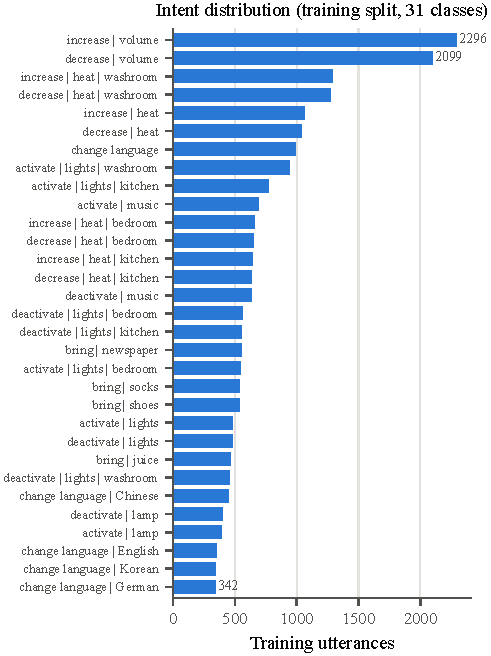
\includegraphics[height=5.5cm]{fig_intent_dist.pdf}
\vspace{-6pt}
\caption{Training utterances per intent.}
\end{figure}
\end{columns}
\end{frame}

%======================================================================
\begin{frame}{Methodology: Overall Flow}
\vspace*{0.05cm}
\begin{figure}
\centering
\resizebox{!}{5.9cm}{% Methodology flow diagram (shared by the report and the slides).
% Requires: tikz with arrows.meta, positioning, fit, backgrounds.
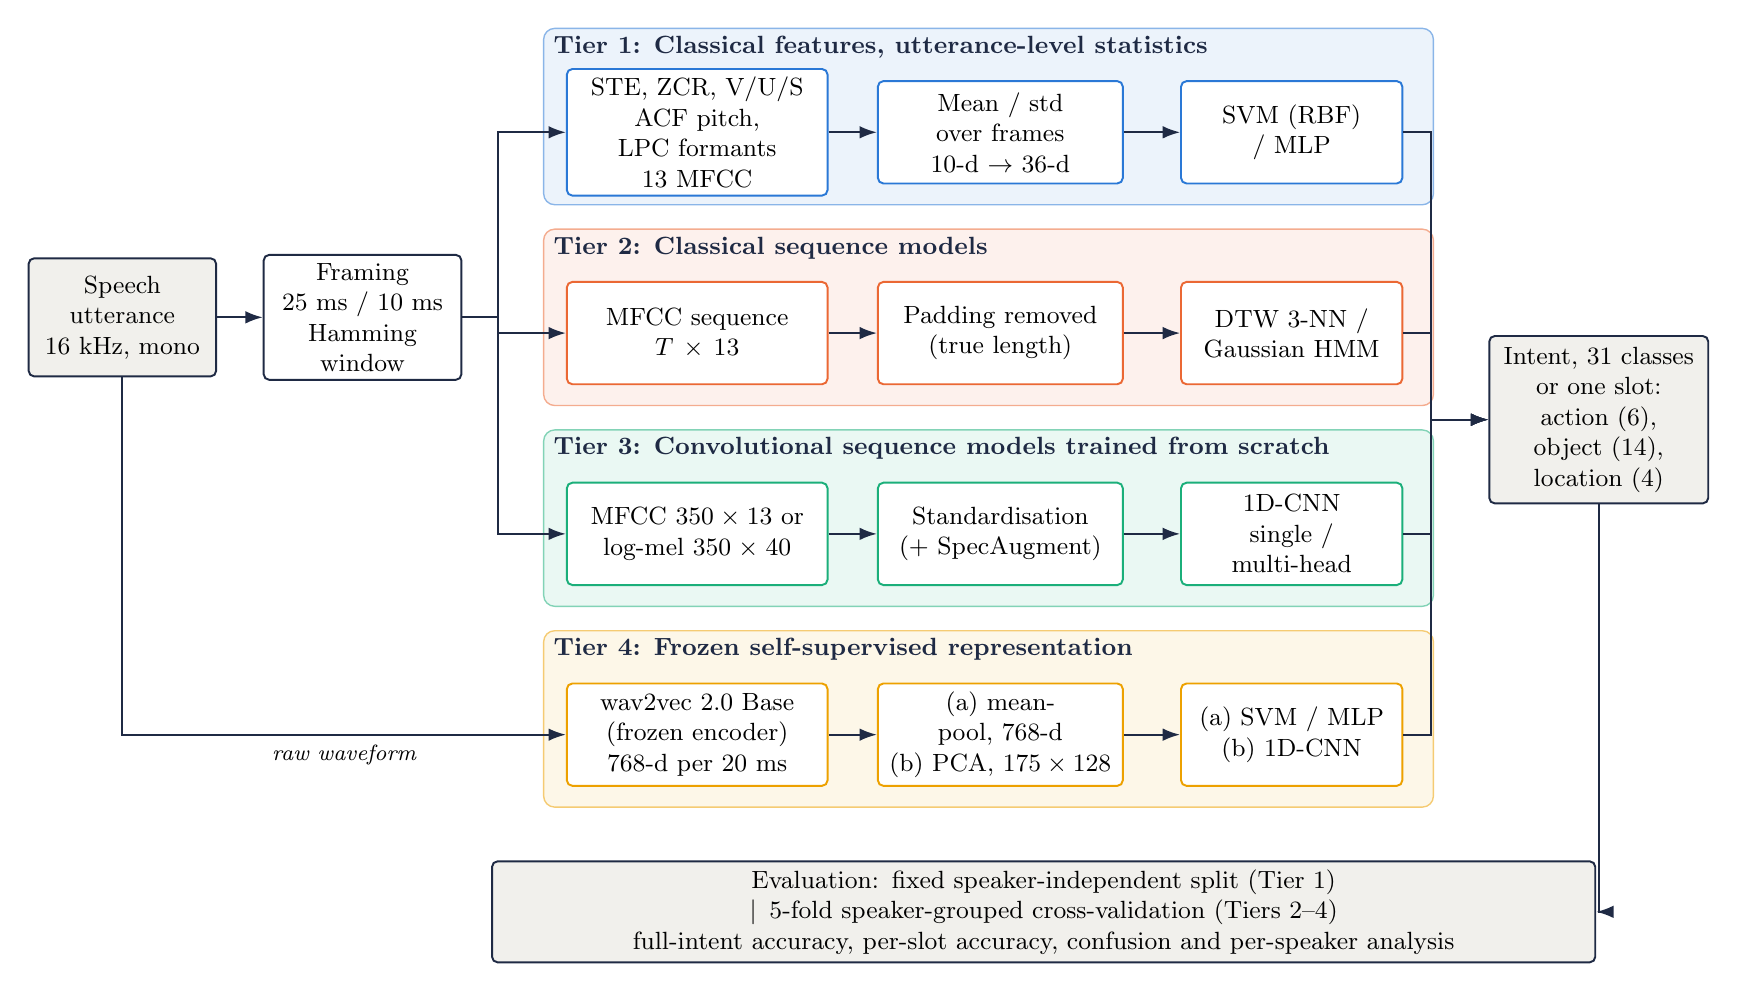
\begin{tikzpicture}[
  font=\small, >={Latex[length=2.2mm,width=1.6mm]},
  box/.style={draw=#1, fill=white, rounded corners=2pt, line width=0.7pt, align=center,
              minimum height=1.3cm, inner sep=3pt},
  io/.style={draw=diagInk, fill=diagGrey, rounded corners=2pt, line width=0.7pt, align=center,
             minimum height=1.5cm, inner sep=4pt},
  band/.style={fill=#1!9, draw=#1!55, rounded corners=4pt, line width=0.5pt},
  tier/.style={font=\small\bfseries, anchor=north west, text=diagInk, inner sep=2pt},
  arr/.style={->, line width=0.7pt, draw=diagInk},
]
% ---------------- tier bands ----------------
\def\tierA{5.1} \def\tierB{2.55} \def\tierC{0.0} \def\tierD{-2.55}
\foreach \y/\c/\t in {\tierA/diagBlue/{Tier 1: Classical features, utterance-level statistics},
                      \tierB/diagOrange/{Tier 2: Classical sequence models},
                      \tierC/diagGreen/{Tier 3: Convolutional sequence models trained from scratch},
                      \tierD/diagYellow/{Tier 4: Frozen self-supervised representation}}{
  \fill[band=\c] (5.05,\y-1.12) rectangle (16.35,\y+1.12);
  \node[tier] at (5.1,\y+1.1) {\t};
}
% ---------------- input and pre-processing ----------------
\node[io, text width=2.1cm] (in) at (-0.3,\tierB) {Speech utterance\\16 kHz, mono};
\node[box=diagInk, text width=2.3cm, minimum height=1.5cm] (pre) at (2.75,\tierB)
     {Framing\\25 ms / 10 ms\\Hamming window};
% ---------------- Tier 1 ----------------
\node[box=diagBlue, text width=3.1cm] (a1) at (7.0,\tierA-0.2) {STE, ZCR, V/U/S\\ACF pitch, LPC formants\\13 MFCC};
\node[box=diagBlue, text width=2.9cm] (a2) at (10.85,\tierA-0.2) {Mean / std\\over frames\\10-d $\rightarrow$ 36-d};
\node[box=diagBlue, text width=2.6cm] (a3) at (14.55,\tierA-0.2) {SVM (RBF) / MLP};
% ---------------- Tier 2 ----------------
\node[box=diagOrange, text width=3.1cm] (b1) at (7.0,\tierB-0.2) {MFCC sequence\\$T \times 13$};
\node[box=diagOrange, text width=2.9cm] (b2) at (10.85,\tierB-0.2) {Padding removed\\(true length)};
\node[box=diagOrange, text width=2.6cm] (b3) at (14.55,\tierB-0.2) {DTW 3-NN /\\Gaussian HMM};
% ---------------- Tier 3 ----------------
\node[box=diagGreen, text width=3.1cm] (c1) at (7.0,\tierC-0.2) {MFCC $350 \times 13$ or\\log-mel $350 \times 40$};
\node[box=diagGreen, text width=2.9cm] (c2) at (10.85,\tierC-0.2) {Standardisation\\(+ SpecAugment)};
\node[box=diagGreen, text width=2.6cm] (c3) at (14.55,\tierC-0.2) {1D-CNN\\single / multi-head};
% ---------------- Tier 4 ----------------
\node[box=diagYellow, text width=3.1cm] (d1) at (7.0,\tierD-0.2) {wav2vec 2.0 Base\\(frozen encoder)\\768-d per 20 ms};
\node[box=diagYellow, text width=2.9cm] (d2) at (10.85,\tierD-0.2) {(a) mean-pool, 768-d\\(b) PCA, $175 \times 128$};
\node[box=diagYellow, text width=2.6cm] (d3) at (14.55,\tierD-0.2) {(a) SVM / MLP\\(b) 1D-CNN};
% ---------------- output and evaluation ----------------
\node[io, text width=2.5cm] (out) at (18.45,1.25) {Intent, 31 classes\\or one slot:\\action (6), object (14),\\location (4)};
\node[box=diagInk, fill=diagGrey, text width=13.8cm, minimum height=0.95cm] (ev) at (11.4,-5.0)
     {Evaluation: fixed speaker-independent split (Tier 1) \,$\vert$\, 5-fold speaker-grouped cross-validation (Tiers 2--4)\\
      full-intent accuracy, per-slot accuracy, confusion and per-speaker analysis};
% ---------------- arrows ----------------
\draw[arr] (in) -- (pre);
\foreach \n in {a1,b1,c1}{ \draw[arr] (pre.east) -- ++(0.45,0) |- (\n.west); }
\draw[arr] (in.south) |- node[pos=0.75, below, font=\footnotesize\itshape] {raw waveform} (d1.west);
\foreach \p/\q in {a1/a2,a2/a3,b1/b2,b2/b3,c1/c2,c2/c3,d1/d2,d2/d3}{ \draw[arr] (\p) -- (\q); }
\foreach \n in {a3,b3,c3,d3}{ \draw[arr] (\n.east) -- ++(0.35,0) |- (out.west); }
\draw[arr] (out.south) |- (ev.east);
\end{tikzpicture}
}
\vspace{-6pt}
\caption{Four representation tiers, ordered from classical to modern.}
\end{figure}
\end{frame}

%======================================================================
\begin{frame}{Methodology: Classical Feature Extraction}
\begin{itemize}\setlength{\itemsep}{5pt}
\item Framing: 25 ms frames (400 samples), 10 ms hop, Hamming window
\item Short-time energy $E_m = \sum_n x_m^2[n]$; ZCR = fraction of sign changes per frame
\item Speech if energy $>$ utterance noise floor + 10 dB; unvoiced if ZCR $>$ 70th percentile
\item Pitch: autocorrelation peak in 70--400 Hz; confidence $r[k^\ast]/r[0] \ge 0.3$
\item Linear prediction: order 16, autocorrelation method, Levinson--Durbin recursion
\item MFCC: mel filter bank $\rightarrow$ log $\rightarrow$ DCT $\rightarrow$ 13 coefficients
\item Log-mel: same pipeline without the DCT, 40 bands
\item Utterance vector: mean / std statistics, 10-d (prosodic) and 36-d (+ MFCC)
\item Full-corpus pitch with YIN \cite{decheveigne2002yin}; same periodicity principle, faster
\end{itemize}
\end{frame}

%======================================================================
\begin{frame}{Methodology: Models and Evaluation Protocol}
\begin{figure}
\centering
\resizebox{0.94\linewidth}{!}{% 1D-CNN used for every sequence experiment (Tiers 3 and 4).
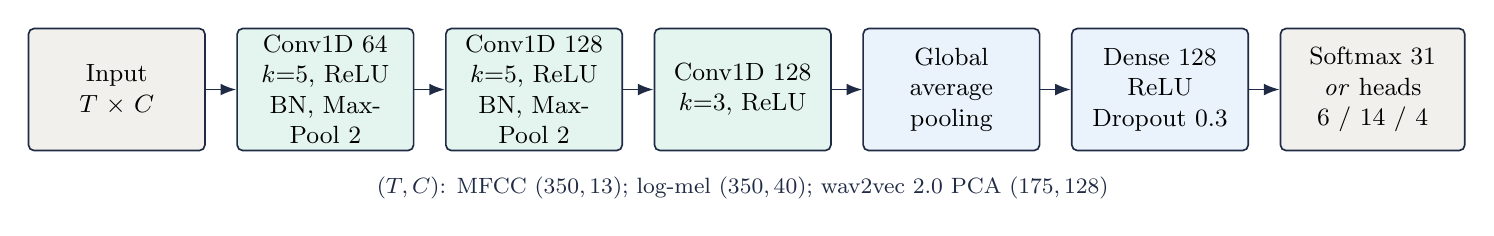
\begin{tikzpicture}[
  font=\small, >={Latex[length=2mm,width=1.5mm]},
  layer/.style={draw=diagInk, fill=#1, rounded corners=2pt, line width=0.6pt, align=center,
                minimum height=1.55cm, text width=2.1cm, inner sep=2pt},
  arr/.style={->, line width=0.7pt, draw=diagInk},
]
\node[layer=diagGrey] (x) at (0,0) {Input\\$T \times C$};
\node[layer=diagGreen!12] (c1) at (2.65,0) {Conv1D 64\\$k{=}5$, ReLU\\BN, MaxPool 2};
\node[layer=diagGreen!12] (c2) at (5.30,0) {Conv1D 128\\$k{=}5$, ReLU\\BN, MaxPool 2};
\node[layer=diagGreen!12] (c3) at (7.95,0) {Conv1D 128\\$k{=}3$, ReLU};
\node[layer=diagBlue!10] (g) at (10.60,0) {Global\\average\\pooling};
\node[layer=diagBlue!10] (d) at (13.25,0) {Dense 128\\ReLU\\Dropout 0.3};
\node[layer=diagGrey, text width=2.2cm] (o) at (15.95,0) {Softmax 31\\\emph{or} heads\\6 / 14 / 4};
\foreach \p/\q in {x/c1,c1/c2,c2/c3,c3/g,g/d,d/o}{ \draw[arr] (\p) -- (\q); }
\node[font=\footnotesize, text=diagInk, align=center] at (7.95,-1.25)
  {$(T,C)$: MFCC $(350,13)$; log-mel $(350,40)$; wav2vec 2.0 PCA $(175,128)$};
\end{tikzpicture}
}
\vspace{-4pt}
\caption{1D-CNN shared by Tiers 3 and 4 (115,871 parameters on MFCC input).}
\end{figure}
\vspace{-6pt}
\small
\begin{itemize}\setlength{\itemsep}{1pt}
\item Tier 1: SVM (RBF) and MLP, grid-searched on the official validation subset
\item Tier 2: DTW 3-NN with 5 templates per intent; 3-state diagonal Gaussian HMM per intent
\item Tier 3: Adam, batch 128, early stopping; multi-head variant adds SpecAugment \cite{park2019specaugment}
\item Tier 4: frozen wav2vec 2.0 Base \cite{baevski2020wav2vec2}; mean-pooled 768-d or PCA-128 sequence
\item Evaluation: same 5 speaker folds for every model and task
\end{itemize}
\end{frame}

%======================================================================
\begin{frame}{Results: Time-Domain Analysis of ``Bring socks''}
\begin{columns}[T]
\column{0.50\textwidth}
\begin{figure}
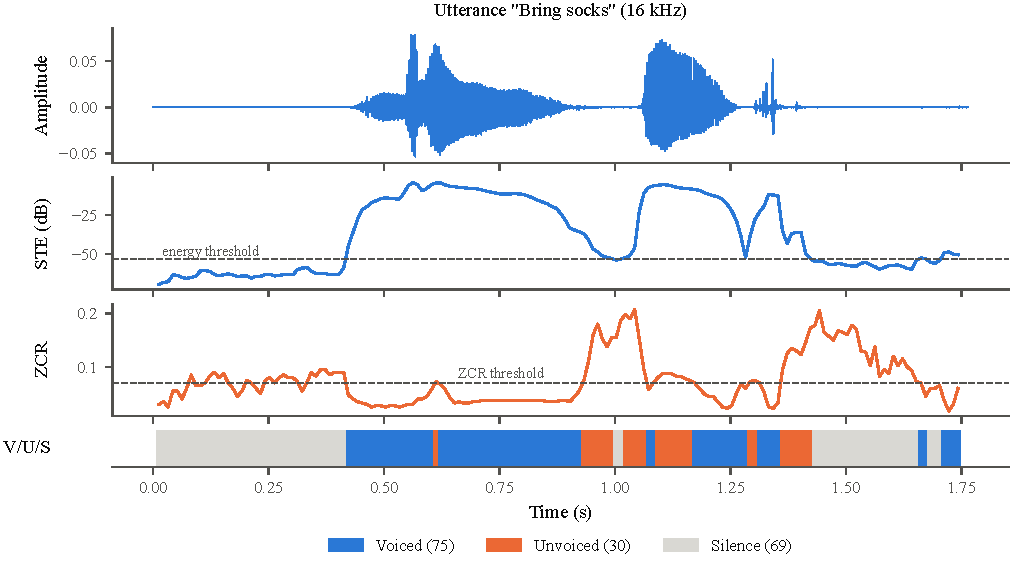
\includegraphics[width=\linewidth]{fig_vus.pdf}
\vspace{-6pt}
\caption{Waveform, STE, ZCR and V/U/S labels.}
\end{figure}
\column{0.48\textwidth}
\begin{figure}
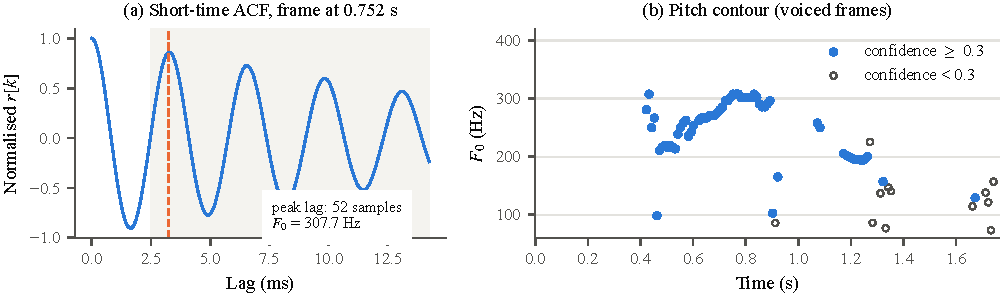
\includegraphics[width=\linewidth]{fig_pitch.pdf}
\vspace{-6pt}
\caption{ACF of a voiced frame and $F_0$ contour.}
\end{figure}
\vspace{-4pt}
\small
\begin{itemize}\setlength{\itemsep}{1.5pt}
\item Frames: 75 voiced, 30 unvoiced, 69 silent
\item /s/: low energy with ZCR of 0.15--0.21
\item /k/ burst shorter than one 25 ms frame
\item $F_0$ 210 $\rightarrow$ 310 Hz on ``bring''
\item 63 of 75 reliable; octave error at 0.463 s
\end{itemize}
\end{columns}
\end{frame}

%======================================================================
\begin{frame}{Results: Spectral Analysis and Linear Prediction}
\begin{columns}[T]
\column{0.56\textwidth}
\begin{figure}
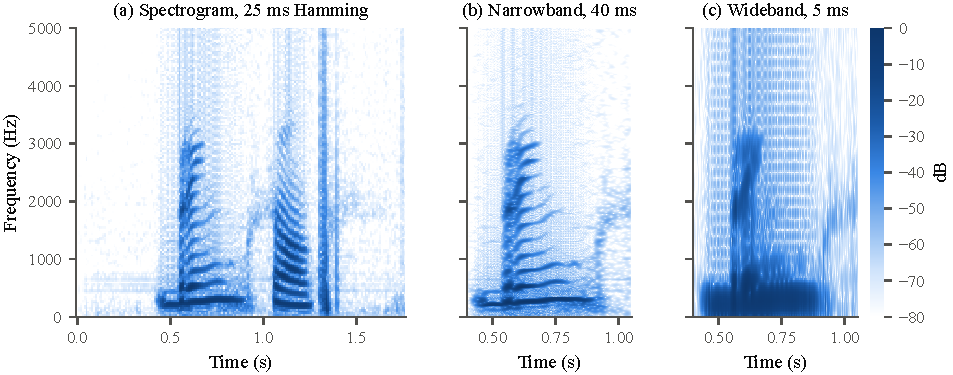
\includegraphics[height=2.45cm]{fig_spectrogram.pdf}
\vspace{-6pt}
\caption{Spectrogram; narrowband vs.\ wideband.}
\end{figure}
\vspace{-8pt}
\begin{figure}
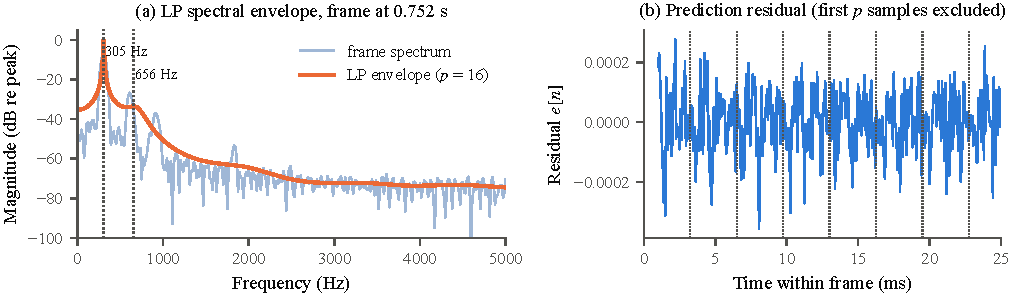
\includegraphics[height=2.2cm]{fig_lpc.pdf}
\vspace{-6pt}
\caption{LP envelope ($p = 16$) and residual.}
\end{figure}
\column{0.41\textwidth}
\vspace{0.5cm}
\small
\begin{itemize}\setlength{\itemsep}{6pt}
\item Harmonic spacing agrees with ACF pitch
\item Fricatives: diffuse energy, no harmonics
\item /k/ release: brief broadband stripe
\item 40 ms resolves harmonics; 5 ms, pulses
\item LP resonances at 305 Hz and 656 Hz
\item Burg-method envelope: same peaks
\item Residual periodicity falls as $p$ rises
\end{itemize}
\end{columns}
\end{frame}

%======================================================================
\begin{frame}{Results: Tier 1, Utterance-Level Statistics}
\begin{columns}[T]
\column{0.56\textwidth}
\scriptsize
\begin{table}
\caption{31-class accuracy (\%): official split and 5-fold speaker CV.}
\begin{tabular}{@{}llrrr@{}}
\toprule
Features & Classifier & Valid. & Test & CV\\
\midrule
-- & Majority & 10.2 & 10.4 & $10.0 \pm 0.2$\\
Prosodic & SVM & 16.4 & 16.5 & $17.8 \pm 1.0$\\
Prosodic & MLP & 15.2 & 14.3 & $16.5 \pm 1.5$\\
+ MFCC & SVM & 22.3 & \textbf{25.8} & $\mathbf{24.0 \pm 1.0}$\\
+ MFCC & MLP & 22.4 & 21.0 & $21.4 \pm 1.0$\\
\bottomrule
\end{tabular}
\end{table}
\small
\begin{itemize}\setlength{\itemsep}{2.5pt}
\item Prosody alone: about 7 points above the majority class
\item Tuning plateaus near 15--16\%: features limit accuracy
\item + MFCC: +6.2 points in every CV fold ($p < 0.001$)
\item Volume intents: 20\% of outputs vs.\ 10.4\% of labels
\item CV confirms the fixed-split conclusions
\end{itemize}
\column{0.41\textwidth}
\begin{figure}
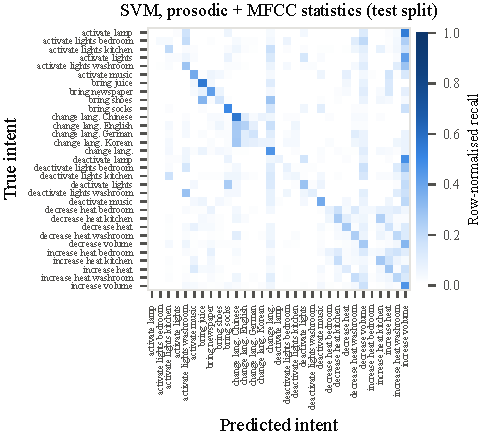
\includegraphics[width=0.96\linewidth]{fig_cm_svm_mfcc.pdf}
\vspace{-6pt}
\caption{SVM on prosodic + MFCC statistics.}
\end{figure}
\end{columns}
\end{frame}

%======================================================================
\begin{frame}{Results: Tier 2, Classical Sequence Models}
\begin{table}
\caption{Accuracy (\%) of the classical sequence classifiers.}
\small
\begin{tabular}{@{}lrl@{}}
\toprule
Model & Accuracy & Evaluation\\
\midrule
Majority class & 10.4 & official test split\\
DTW, 3-nearest neighbours & 11.6 & 155 queries, one fold\\
Gaussian HMM, padded input & $9.8 \pm 0.1$ & 5-fold speaker-grouped CV\\
Gaussian HMM, padding removed & $6.0 \pm 0.7$ & 5-fold speaker-grouped CV\\
\bottomrule
\end{tabular}
\end{table}
\begin{itemize}\setlength{\itemsep}{4pt}
\item Both baselines lie near or below the majority class
\item Padded HMM exploited padding length, an indirect duration cue
\item After padding removal, spectral discrimination alone gives 6.0\%
\item HMM kept minimal: 3 ergodic states, one Gaussian, no delta features
\item DTW used only 5 templates per intent against 248 phrasings
\item Result reflects the minimal configuration, not the classical method itself
\end{itemize}
\end{frame}

%======================================================================
\begin{frame}{Results: Tier 3, CNNs Trained from Scratch}
\begin{columns}[T]
\column{0.57\textwidth}
\scriptsize
\begin{table}
\caption{5-fold speaker-grouped CV, 31-class accuracy (\%).}
\begin{tabular}{@{}lrr@{}}
\toprule
Input / model & Dim. & Mean $\pm$ s.d.\\
\midrule
\multicolumn{3}{@{}l}{\emph{1. Input representation (single head)}}\\
MFCC & 13 & $72.5 \pm 5.0$\\
Log-mel & 40 & $\mathbf{79.4 \pm 6.8}$\\
DCT of log-mel, first 13 & 13 & $73.1 \pm 5.8$\\
DCT of log-mel, all 40 & 40 & $63.5 \pm 5.0$\\
\midrule
\multicolumn{3}{@{}l}{\emph{2. Output structure (MFCC input)}}\\
Multi-head + SpecAugment & 13 & $77.3 \pm 6.7$\\
\bottomrule
\end{tabular}
\end{table}
\small
\begin{itemize}\setlength{\itemsep}{2pt}
\item Same MFCC frames, order kept: 24.0 $\rightarrow$ 72.5\%
\item Log-mel beats MFCC in every fold (+6.9, $p = 0.005$)
\item Full DCT: $-$15.9 points (weak coefficients inflated)
\end{itemize}
\column{0.40\textwidth}
\begin{figure}
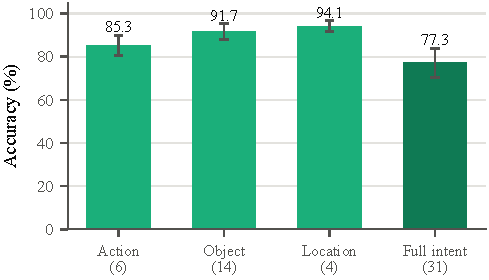
\includegraphics[width=\linewidth]{fig_multihead_slots.pdf}
\vspace{-6pt}
\caption{Multi-head CNN accuracy per slot.}
\end{figure}
\small
\begin{itemize}
\item Multi-head: +4.8 over MFCC, every fold
\item Action is the weakest slot (85.3\%)
\item vs.\ log-mel: n.s.\ ($p = 0.16$)
\end{itemize}
\end{columns}
\end{frame}

%======================================================================
\begin{frame}{Results: Tier 4, Frozen wav2vec 2.0}
\begin{columns}[T]
\column{0.44\textwidth}
\scriptsize
\begin{table}
\caption{This work (5-fold speaker-grouped CV).}
\begin{tabular}{@{}lr@{}}
\toprule
Downstream classifier & Acc. (\%)\\
\midrule
Mean-pooled + SVM & $59.9 \pm 4.4$\\
Mean-pooled + MLP & $69.9 \pm 4.7$\\
Frame sequence + 1D-CNN & $\mathbf{93.1 \pm 3.1}$\\
\bottomrule
\end{tabular}
\end{table}
\vspace{-4pt}
\begin{table}
\caption{Published FSC results (official test split).}
\begin{tabular}{@{}lr@{}}
\toprule
Model & Acc. (\%)\\
\midrule
wav2vec 2.0 Base, frozen \cite{yang2021superb} & 92.35\\
HuBERT Base, frozen \cite{yang2021superb} & 98.34\\
ASR pre-trained, frozen \cite{lugosch2019fsc} & 98.8\\
End-to-end transformer \cite{radfar2020transformer} & 99.6\\
\bottomrule
\end{tabular}
\end{table}
\column{0.53\textwidth}
\vspace{0.3cm}
\small
\begin{itemize}\setlength{\itemsep}{7pt}
\item Pooling discards order: pooled MLP $\approx$ MFCC CNN
\item Frame sequence + CNN: best model in every fold
\item +13.7 points over the log-mel CNN ($p = 0.001$)
\item Lowest fold-to-fold spread of all models
\item Close to SUPERB frozen wav2vec 2.0 Base (92.35\%)
\item Gap to 98--99.6\%: last layer only \cite{pasad2021layerwise}, PCA, frozen
\end{itemize}
\end{columns}
\end{frame}

%======================================================================
\begin{frame}{Results: Overall Comparison}
\begin{figure}
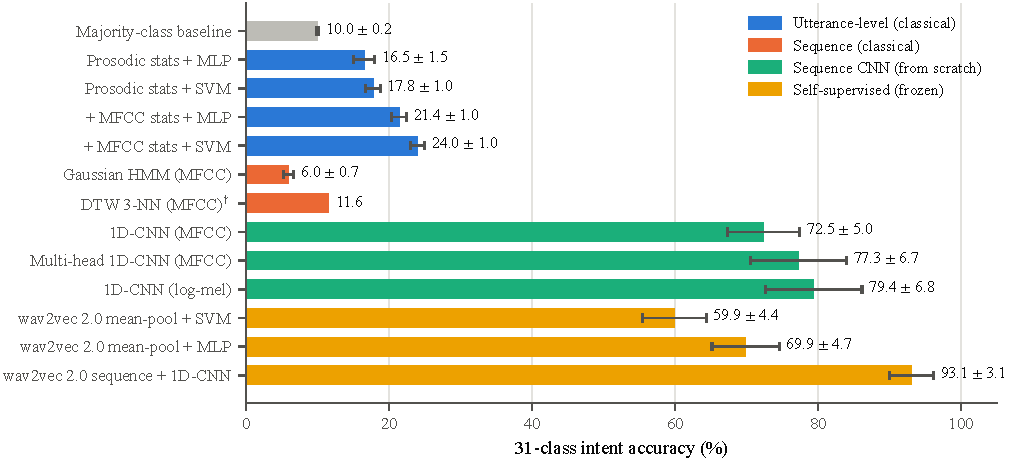
\includegraphics[height=4.3cm]{fig_overall.pdf}
\vspace{-6pt}
\caption{All configurations under 5-fold speaker CV, classical to modern ($^{\dagger}$155-query subset).}
\end{figure}
\vspace{-6pt}
\small
\begin{columns}[T]
\column{0.47\textwidth}
\begin{itemize}\setlength{\itemsep}{1pt}
\item Cepstral content: 17.8 $\rightarrow$ 24.0\%
\item Temporal order: 24.0 $\rightarrow$ 72.5--79.4\%
\end{itemize}
\column{0.47\textwidth}
\begin{itemize}\setlength{\itemsep}{1pt}
\item Self-supervised frames: 79.4 $\rightarrow$ 93.1\%
\item All tiers on the same speaker folds
\end{itemize}
\end{columns}
\end{frame}

%======================================================================
\begin{frame}{Results: Reduced-Class Slot Tasks}
\begin{figure}
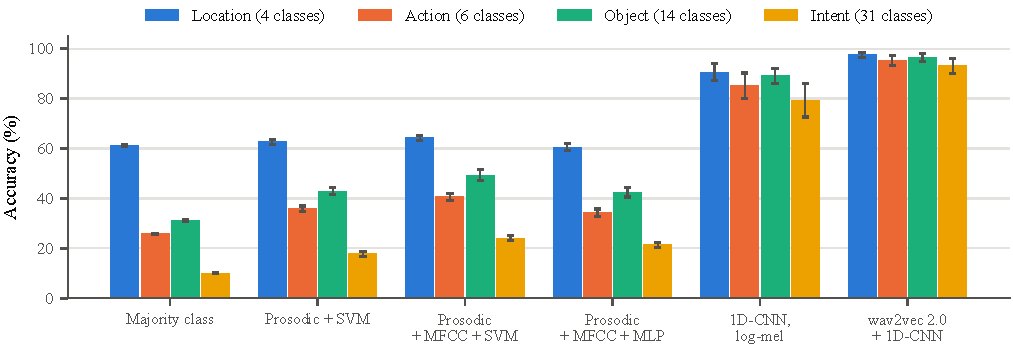
\includegraphics[height=3.85cm]{fig_slot_tasks.pdf}
\vspace{-6pt}
\caption{Accuracy per task under 5-fold speaker CV (classes: location 4, action 6, object 14, intent 31).}
\end{figure}
\vspace{-8pt}
\small
\begin{columns}[T]
\column{0.49\textwidth}
\begin{itemize}\setlength{\itemsep}{1pt}
\item Fewer classes raise accuracy for every model
\item Majority baseline also rises: 10.0 $\rightarrow$ 25.8--61.2\%
\item SVM removes only 8--26\% of the majority error
\end{itemize}
\column{0.49\textwidth}
\begin{itemize}\setlength{\itemsep}{1pt}
\item Location: MLP below majority (60.5 vs.\ 61.2\%)
\item CNNs remove 76--95\% of the majority error
\item Limit is the representation, not the class count
\end{itemize}
\end{columns}
\end{frame}

%======================================================================
\begin{frame}{Results: Error and Speaker Variability Analysis}
\begin{columns}[T]
\column{0.38\textwidth}
\begin{figure}
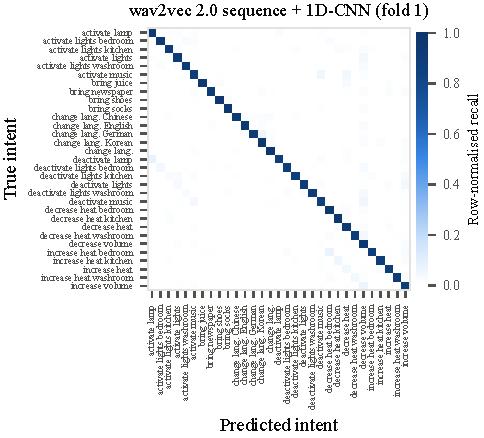
\includegraphics[width=\linewidth]{fig_cm_w2v.pdf}
\vspace{-6pt}
\caption{wav2vec 2.0 + CNN, fold 1 (91.7\%).}
\end{figure}
\column{0.59\textwidth}
\begin{figure}
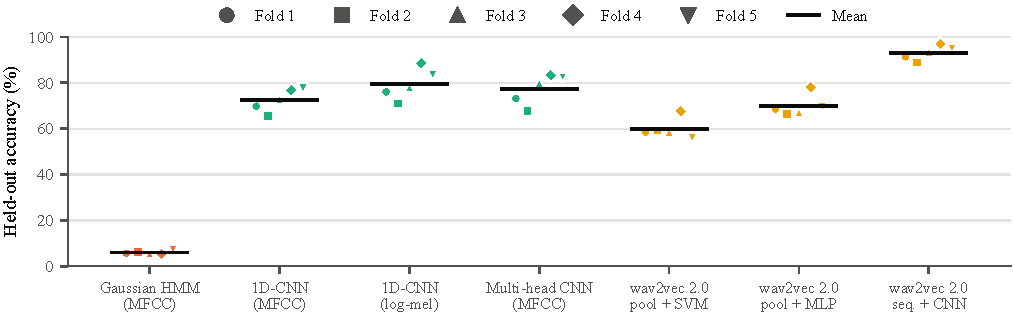
\includegraphics[width=\linewidth]{fig_folds.pdf}
\vspace{-6pt}
\caption{Held-out accuracy per fold.}
\end{figure}
\vspace{-6pt}
\small
\begin{itemize}\setlength{\itemsep}{1.5pt}
\item Slot accuracy: action 93.9, object 95.2, location 97.2\%
\item Top confusion: increase $\rightarrow$ decrease volume (40 errors)
\item Polarity often rests on one particle: \emph{up/down}, \emph{on/off}
\item Speakers: 36.4--100\% accuracy; 14 of 19 above 89\%
\end{itemize}
\end{columns}
\end{frame}

%======================================================================
\begin{frame}{Conclusion and Future Work}
\begin{columns}[T]
\column{0.53\textwidth}
\textbf{Conclusion}
\small
\begin{itemize}\setlength{\itemsep}{3.5pt}
\item Pitch, spectral and LP analyses agree with each other
\item Prosodic statistics alone give only 17.8\%
\item MFCC statistics recover part of the gap (24.0\%)
\item Keeping temporal order gives the largest gain
\item DCT + standardisation hurts the CNN; log-mel is better
\item Frozen wav2vec 2.0 + CNN is best: 93.1 $\pm$ 3.1\%
\item Slot tasks: classical stays near majority; CNNs 85--97\%
\item Residual errors: opposite-polarity commands
\item FSC needs speaker-grouped CV, not one split
\end{itemize}
\column{0.44\textwidth}
\textbf{Future Work}
\small
\begin{itemize}\setlength{\itemsep}{3.5pt}
\item Left-to-right GMM-HMM with deltas \cite{furui1986delta}
\item Learned wav2vec 2.0 layer weighting \cite{yang2021superb}
\item HuBERT and encoder fine-tuning \cite{hsu2021hubert}
\item Robustness to noise and unseen phrasings
\end{itemize}
\end{columns}
\end{frame}

%======================================================================
\begin{frame}[allowframebreaks]{References}
\fontsize{5.6}{6.5}\selectfont
\bibliographystyle{IEEEtran}
\bibliography{refs}
\end{frame}


\end{document}
